\clearpage
\chapter{Finite Element Method}

This paper focuses its mathematics on implementing the finite element method to solve PDEs. This chapter will go through the necessary mathematics behind each of the steps in the finite element method such as variational calculus, approximation theory and finite elements themselves. The chapter also goes through the approach itself, alongside the worked example for the case of this study of the Laplace equation.

\section{General Problem}

Before the nuts and bolts of the finite element method are discussed, first consider an $n$-dimensional, general $n$\textsuperscript{th} order PDE of the form,
\begin{equation}
	f\left(\mathbf{x}; u(\mathbf{x}), \frac{\partial u}{\partial x_1},\dots, \frac{\partial u}{\partial x_n}; \frac{\partial^2 u}{\partial x_1 \partial x_1},\dots,\frac{\partial^2 u}{\partial x_i \partial x_j},\dots, \frac{\partial^2 u}{\partial x_n \partial x_n}; \dots\right) = 0,
\end{equation}
where $\mathbf{x} = \{x_1,x_2,\dots,x_n\}$.
For a case of a 2-dimensional, 2\textsuperscript{nd} order PDE, this results in ending up with the operator,
\begin{equation}
	\mathcal{L} = a \frac{\partial^2}{\partial x^2} + b \frac{\partial^2}{\partial x \partial y} + c \frac{\partial^2}{\partial y^2} + F\left(x,y; \frac{\partial}{\partial x}, \frac{\partial}{\partial y}\right).
\end{equation}
This can be used, by applying it to a function $u(\mathbf{x})$, leaving a PDE,
\begin{equation}\label{pde}
	\mathcal{L}u = 0,
\end{equation}
which is going to be basis for this study - attempting to approximate the function $u(\mathbf{x})$. This problem can then be bounded by three types of non-homogeneous boundary conditions in order to be properly posed and have a unique/non-trivial solution:
\begin{enumerate}
	\item Dirichlet condition: $u=g(s)$.
	\item Neumann condition: $\frac{\partial u}{\partial \mathbf{n}} = h(s)$.
	\item Robin condition: $\frac{\partial u}{\partial \mathbf{n}} + \sigma(s)u = k(s)$,
\end{enumerate}
where $s$ is the arc length of the boundary $C$ and $\mathbf{n}$ is a vector, externally normal to $C$.~\cite{davies} How these conditions are imposed and handled is discussed in Section~\ref{boundaries}, later in the report.

\section{Approximation Theory}

Suppose there exists some function $u(x)$ which is required to be approximated. The most common way to is to estimate the value of the function is by using a collection of \textit{basis functions} $\psi_i(x)$, and unknown coefficients, $c_i$, giving,
\begin{equation}\label{uapprox}
	u(x) \approx \sum_{i=0}^N c_i\psi_i(x).
\end{equation}
There are a collection of ways to construct your basis functions and create a linear system, and obtain solutions to the approximation Equation~\eqref{uapprox} and this paper looks at three in particular:
\begin{itemize}
	\item least squares.
	\item Galerkin.
	\item weighted residuals.
\end{itemize}
There are other methods of approximation such as collocation and regression but they are not discussed here. Before these approaches are explained, two things must first be defined. Firstly, consider a function space $V$, defined by the span of set of basis functions,
\begin{equation}
	V = \text{span}\{\psi_0,\dots,\psi_N\},
\end{equation}
then it can be said the any function $u\in V$ can be written as a linear combination of the basis functions,
	\begin{equation}\label{basis}
		u(x) = \sum_i c_i \psi_i. 
	\end{equation}
\cite{mardal}. Consider now, functions $f,g$ - the squared-norm or inner-product of these two functions is defined as,
\begin{equation}\label{innerprod}
	\langle f,g\rangle = \int f(x)g(x)dx
\end{equation}

\subsection{Least Squares}

Consider a function $f(x)$ which needs to be approximated by a function $u(x)$ $\in V$ as defined in Equation~\eqref{basis}. The most obvious way to approximate this function would be to minimise the differential between the two, $f-u$. Subbing this into the inner product defined in Equation~\eqref{innerprod} leaves the error,
\begin{align}
	e &= \langle f-u, f-u\rangle = \langle f-\sum_i c_i \psi_i,f-\sum_i c_i \psi_i\rangle,\\
	e &= \langle f,f\rangle - 2~\sum_i c_i\langle f,\psi_i\rangle + \sum_{i,j} c_i c_j \langle\psi_i, \psi_j\rangle. 
\end{align}
Of course, now, as is well known from optimisation, to minimise this residual function, its derivative must be taken at each of the $N$ points, $\left\{\frac{\partial e}{\partial c_i}\right\}_N$. Evaluating and setting $\frac{\partial e}{\partial c_i} = 0$, results in the equation,
\begin{equation}
	- \langle f,\psi_i\rangle + \sum_j c_j\langle \psi_i, \psi_j\rangle = 0,\quad i \in \{0,\dots,N\},
\end{equation}
which can equally be written as,
\begin{equation}
	\sum_j A_{i,j}c_j = b_i,
\end{equation}
where,
\begin{align}
	A_{i,j} &= \langle \psi_i, \psi_j\rangle,\\
	b_i &= \langle f, \psi_i \rangle.
\end{align}
Now there is a system of linear equations which can be solved by usual means to obtain the approximation $u(x)$ of the function $f(x)$. Mathematically, it is equivalent to say that the method of least squares utilises the inner-product of the residuals, and solves by minimising it,
\begin{equation}
	\min_{c_0,\dots,c_N} \langle e, e\rangle,
\end{equation}
giving the system of $N+1$ equations,
\begin{equation}
	\left\langle e, \frac{\partial e}{\partial c_i}\right\rangle = 0, \quad i\in\{1,\dots,N\}.
\end{equation}
\cite{mardal}

\subsection{Galerkin}

In the previous subsection, it was shown that the least squares method operates by minimising the error term between the two functions, or alternatively, forcing the error to be orthogonal to the function space $V$. However, in reality, the true error is not actually known, since $f$ is not explicitly known, and thus instead a residual $R$ is used. Take for example, Equation~\eqref{pde}, if we sub in an approximation $\hat{u} = \sum_i c_i \psi_i$, we get,
\begin{equation}
	R = \mathcal{L}\left(\sum_i c_i \psi_i\right) \neq 0.
\end{equation}
Now, the residual $R$ can be made orthogonal to the space $V$ by imposing,
\begin{equation}
	\langle R, v \rangle=0,\quad\forall v \in V,
\end{equation}
and since any function in $V$ can be approximated using Equation~\eqref{basis}, it can be said that,
\begin{equation}
	\langle R, \psi_i \rangle=0,\quad i\in\{1,\dots,N\},
\end{equation}
thus leaving another system of linear equations to solve. This is alternatively known as projecting $R$ onto $V$.
\cite{mardal}

\subsection{Weighted Residuals}\label{residuals}

The method of weighted residuals is a relatively simple generalisation of the standard Galerkin method. Rather than imposing that the residual is orthogonal to the space $V$ known as the trial space, it is chosen to be orthogonal to some alternate space $W$, known as the test space. This leaves the equation,
\begin{equation}
	\langle R, v \rangle=0,\quad \forall v \in W,
\end{equation}
where,
\begin{equation}
	W = \text{span}\{w_0,\dots,w_n\}
\end{equation}
and so this leaves,
\begin{equation}
	\langle R, w_i \rangle=0,\quad i\in\{1,\dots,N\},
\end{equation}
again, leaving a linear system of $N+1$ equations.
\cite{mardal}

\section{Variational Calculus}

\subsection{Weak Formulation}

As it should be clear by now, the overall aim of the finite element method is the minimise a residual in order to get an approximation of the function $u$ as seen in Equation~\eqref{pde}. What may not seem immediately obvious at a first glance, but an important thing to factor in, Equation~\eqref{pde} is not how the PDE problem is posed when trying to apply FEM. In fact, usually, the problem is posed in its \textit{weak formulation}. The weak form of this equation is one which contains at most, first-order derivatives, as opposed to its strong form containing second-order derivatives. When only approximating a normal function defined in a Hilbert space, this issue wouldn't crop up. However, when dealing with calculus of variations, one must remember that boundary conditions must be imposed and reducing the order of derivatives weakens the demands on the test and trial functions, allowing them to not need be continuous in their second derivative.

Take for example a general PDE defined,
\begin{align}
	\mathbf{v}\cdot\nabla u + \beta u &= \nabla\cdot(\alpha\nabla u) + f,\quad  \mathbf{x} \in \Omega \\
	u &= u_D,\quad \mathbf{x} \in \Gamma_D\\
	-\alpha\frac{\partial u}{\partial \mathbf{n}} &= g,\quad \mathbf{x} \in \Gamma_N,
\end{align}
multiplying this by a test function $v$, and getting the inner product over the domain $\Omega$, just like was seen in the method of weighted residuals leaves the equation,
\begin{equation}\label{green}
		\int_{\Omega}(\mathbf{v}\cdot\nabla u + \beta u)v~d\mathbf{x} = \int_{\Omega}\nabla\cdot(\alpha\nabla u)v~d\mathbf{x} + \int_{\Omega}fv~d\mathbf{x}.
\end{equation}
Applying Green's lemma to the second-order term then results in the following equation,
\begin{equation}
	\int_{\Omega}\nabla\cdot(\alpha\nabla u)v~d\mathbf{x} = -\int_{\Omega}\alpha\nabla u\cdot \nabla v~d\mathbf{x} + \oint_{\Gamma} \alpha \frac{\partial u}{\partial \mathbf{n}} v~ds + \int fv~d\mathbf{x}.
\end{equation}
Since the boundary integral is $0$ on $\Gamma_D$ and $g$ on $\Gamma_N$, this can be rewritten as,
\begin{equation}
	\int_{\Omega}\nabla\cdot(\alpha\nabla u)v~d\mathbf{x} = -\int_{\Omega}\alpha\nabla u\cdot \nabla v~d\mathbf{x} + \oint_{\Gamma_N} gv~ds + \int fv~d\mathbf{x},
\end{equation}
and the Equation~\eqref{green} can be shown in terms of the inner product defined in Equation~\eqref{innerprod},
\begin{equation}\label{weak}
	\left\langle\mathbf{v}\cdot\nabla u,v\right\rangle + \left\langle\beta u,v\right\rangle = -\left\langle\alpha\nabla u, \nabla v\right\rangle + \left\langle g,v\right\rangle_N + \left\langle f,v\right\rangle.
\end{equation}
This PDE has now been transformed into its weak formulation. Looking at the Section~\ref{residuals}, it's quite obvious now that $u$ can be approximated by subbing in an estimate, applying the method of weighted residuals and achieving a system of linear equations. Thus the solution space has been reduced to a finite dimensional space.
\cite{mardal}

\subsection{Functionals}\label{functionals}

While regular calculus deals with changes in ordinary variables, calculus of variations by contrast deals with changes in functions - handling special functions  known as functionals, which take functions as inputs compared to just variables. These are beneficial for the FEM as, considering the problem posed in the previous section, much of what is trying to be accomplished is finding the function which minimises an integral i.e. minimising a functional. Take for example, the functional 
\begin{equation}
	F[y(x)] = \int_\Omega f(x, y(x),y'(x))~dx,
\end{equation}
in this instance, one would search for what function $y(x)$ would minimise the integral.

Before discussing how to derive these functionals, first look at an abstract notation for variational forms discussed in the previous sections. Take a function with trial functions $u$, and test functions $v$, supported on $V$, then define the problem as,
\begin{equation}
	a(u,v) = L(v),\quad v\in V,
\end{equation}
where $a(u,v)$ is in bilinear form, containing all terms which have both test and trial functions, whereas, $L(v)$ is linear, containing only test functions. This is equivalent to the integrals seen in Equation~\eqref{weak}, which is looked to be to minimised. This equation is equivalent to minimising the functional,
\begin{equation}\label{func_min}
	I[v] = \frac{1}{2}a(u,v) - L(v). 
\end{equation}
In a multidimensional case, consider the PDE,
\begin{align}
	-\nabla(\alpha\nabla u) + \beta u &= f,\quad \mathbf{x} \in \Omega\\
	u &= u_D,\quad \mathbf{x} \in \Gamma_D\\
	-\alpha \frac{\partial u}{\partial \mathbf{n}} + \sigma(s) u &= k,\quad \mathbf{x}\in \Gamma_R	
\end{align}
Applying the minimisation seen in equation~\eqref{func_min}, and applying some standard multivariable calculus, the resulting functional is,
\begin{equation}
	I[u] = \int_\Omega (\nabla u\cdot \alpha \nabla u) + \beta u^2 - 2 u f)~d\mathbf{x} + \oint_{\Gamma_R} (\sigma u^2 - 2 u k)~ds
\end{equation}
These functionals are an alternative and mathematically equivalent variant on attempting to minimising the problem at hand and a commonly seen in papers discussing the FEM. \cite{davies}

\section{Finite Elements}\label{elems}

Up to this point, the basis functions that have been used have all been defined across the entire domain $\Omega$. In this section, piecewise polynomial basis functions will be used, defined with \textit{compact support} across what are known as \textit{elements} or \textit{cells}. These cells will contribute their own weighted value to the linear system in an assembly process, generating an overall linear system $Lu = b$, where $L$ is known as the global stiffness matrix and $b$ the stress vector. This system will result in the solution to the PDE problem at hand.

\begin{remark}
	As is convention in the FEM to refer to basis functions as $\varphi(x)$, from here on out in the paper, $\psi_i(x)$ will be replaced by $\varphi_i(x)$ - though note they are completely equivalent.
\end{remark}

\subsection{Cells \& Basis Functions}

\begin{figure}
	\centering
	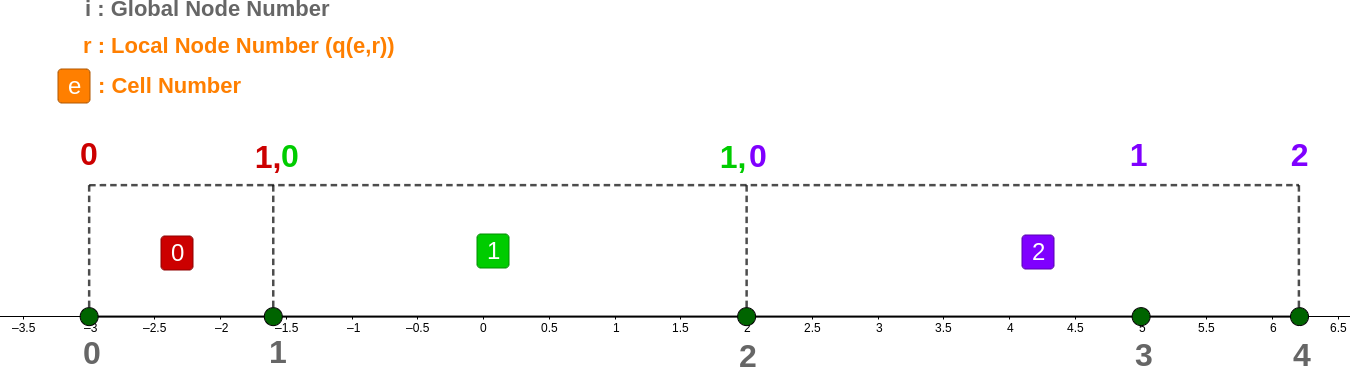
\includegraphics[width=0.8\linewidth]{Figures/node_numbers}
	\caption{Illustration of three cell, 1D mesh with $\Omega_0 = \{0,1\},~\Omega_1 = \{1,2\},~\Omega_2 = \{2,3,4\}$.}
	\label{fig:cells}
\end{figure}
\begin{figure}
	\centering
	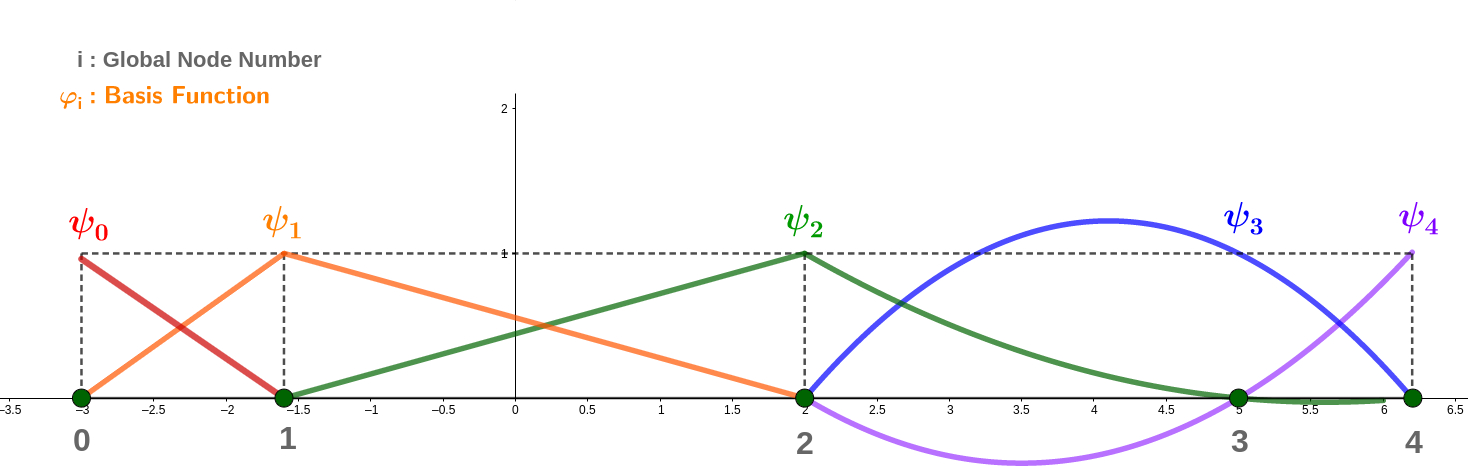
\includegraphics[width=0.8\linewidth]{Figures/basis_funcs}
	\caption{1D mesh representation, with 1\textsuperscript{st} order (P1) Lagrange polynomials in cells 0,1 and 2\textsuperscript{nd} (P2) order in cell 2.}
	\label{fig:1dbasis}
\end{figure}
For illustrative purposes, a single-dimensional problem is used here to demonstrate the actual concept of the finite elements or cells. Consider now a domain,
\begin{equation}
	\Omega = \Omega^{(0)}\cup\Omega^{(1)}\cdots\Omega^{(N_e)},
\end{equation}
where 
\begin{equation}
	\Omega^{(i)}\cap\Omega^{(j)} = \emptyset \quad \forall i,j \in \{0,\dots,N_e\}.
\end{equation}
Within this domain, define $N_n$ nodes, spaced out across the domain any particular amount. Suppose a node has a \textit{global index} $i \in \{0,\dots,N_n\}$ and are laid out in no particular order. We define the node's \textit{local index} in cell $e$ as $r \in \{0,\dots,d\}$, again these do not need to necessarily be in order or equally spaced. Now that the local and global numbering of the nodes are defined, we define the function,
\begin{equation}\label{dof}
	i = q(e,r),
\end{equation}
where $q(e,r)$ is a mapping function from local index $r$ in cell $e$, back to the node's global index across the domain. Figure~\ref{fig:cells} demonstrates these definitions for a simple, three cell, 1D case. Basis functions must next be defined across the domain in order to make an approximation for $u$. Consider a node, globally numbered $i$, locally numbered $r$, on cell $e$, with $d+1$ nodes in said cell, its corresponding basis function $\varphi_i(x)$ is defined as a Lagrange polynomial of degree $d$,
\begin{equation}
	l_d(x) = \prod_{\substack{0\leq m\leq k \\ m\neq j}}\frac{x-x_m}{x_j-x_m} 
\end{equation}
which is $1$ at node $r$ and $0$ everywhere else. If the node is internal, then the function is simply defined as is, if the node is shared with a neighbouring cell, then the basis function is a piecewise combination of the Lagrange polynomial from both cells which share the node. The value $d$ is known as the degree of freedom and is related to the order of polynomial used as the basis function - the higher the order, the more nodes per cell. More often than not, cells are made up into triangular or tetrahedral shapes. However, they can be any shape such as squares or octagons, so long as the degree of freedom mapping is correct. Figures~\ref{fig:1dbasis},~\ref{fig:2dbasis} illustrate these piecewise polynomials in both 1D and 2D. Now it can be said that
\begin{equation}\label{femapprox}
	u(x) \approx \sum_{\mathcal{I}_s} c_i \varphi_i(x),
\end{equation}
where $\mathcal{I}_s$ is the set of indices for which $u(x_i)$ is unknown.
\cite{strang}

\begin{figure}
	\centering
	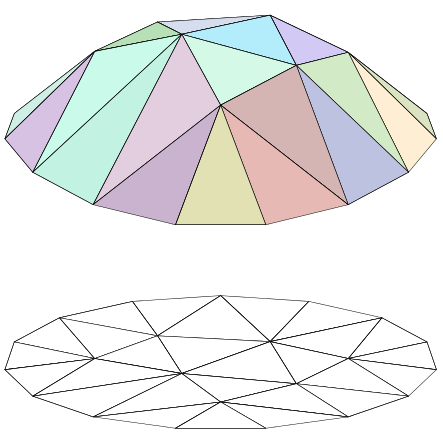
\includegraphics[width=0.4\linewidth]{Figures/Piecewise_linear_function2D}
	\caption{2D mesh representation of P1 basis functions.}
	\label{fig:2dbasis}
\end{figure}

\subsection{Assembling the Stiffness Matrix}

The next piece to the FEM puzzle is a linear system must be assembled from these basis functions in order to solve for the unknowns $\{c_i\}_{\mathcal{I}_s}$ and achieve an approximation for $u$. It was shown in Section~\ref{functionals}, that a variational form PDE can be written in an abstract form as,
\begin{equation}
	a(u,v) = L(v),\quad v\in V.
\end{equation}
With that in mind, consider the PDE from Equation~\eqref{weak}, moving all the terms with both test and trial function to the left-hand side, this can be rewritten as,
\begin{equation}
	\left\langle\mathbf{v}\cdot\nabla u,v\right\rangle + \left\langle\beta u,v\right\rangle + \left\langle\alpha\nabla u, \nabla v\right\rangle = \left\langle g,v\right\rangle_N + \left\langle f,v\right\rangle,
\end{equation}
or subbing in Equation~\eqref{femapprox}, leaves,
\begin{equation}\label{linsys}
	\sum_{\mathcal{I}_s}\left(\left\langle\mathbf{v}\cdot\nabla \varphi_j,\varphi_i\right\rangle + \left\langle\beta \varphi_j,\varphi\right\rangle + \left\langle\alpha\nabla \varphi_j, \nabla \varphi_i\right\rangle\right)c_j = \left\langle g,\varphi_i\right\rangle_N + \left\langle f,\varphi_i\right\rangle,
\end{equation}
which clearly demonstrates a linear system,
\begin{equation}
	\sum_{\mathcal{I}_s} A_{i,j}c_j = b_i,
\end{equation}
where,
\begin{align}
	A_{i,j} &= \left\langle\mathbf{v}\cdot\nabla \varphi_j,\varphi_i\right\rangle + \left\langle\beta \varphi_j,\varphi_i\right\rangle + \left\langle\alpha\nabla \varphi_j, \nabla \varphi_i\right\rangle,\\
	b_i &= \left\langle g,\varphi_i\right\rangle_N + \left\langle f,\varphi_i\right\rangle.
\end{align}
Equation~\eqref{linsys} shows clearly now why it was important to convert the PDE into its weak formulation. Now there are only first-order derivatives of the basis and trial functions which need to be continuous. Had it been left in strong form these would have been second-order.

This has now shown how the overall stiffness matrix would be calculated over the entire domain $\Omega$, but is this achieved this from the elements and their basis functions? The main sell of the FEM is that the domain can be decomposed into elements with easier to evaluate integrals and are robustly able to form many complex overall domain shapes, and then assemble these results into the global stiffness matrix. Remembering that these basis functions are compactly supported, it can be seen that $A_{i,j}$ can be assembled by incrementing the integral result from all cells which contain nodes $i,j$  i.e.
\begin{align}
	A_{i,j} &\coloneqq A_{q(e,r),q(e,s)} + \widetilde{A}_{r,s}^{(e)} \label{aij}\\
	b_i &\coloneqq b_{q(e,r)} + \widetilde{b}_r^{(e)},				\label{bi}
\end{align}
where $\widetilde{\mathbf{A}}^{(e)}$ and $\widetilde{\mathbf{b}}^{(e)}$ are known as the element matrix and element vector, respectively, and $r,s$ are local node numberings as defined in Equations~\eqref{dof}. Both of these evaluate the same integrands, but over their compact support instead of the entire domain. Thus, looking at Equations~\eqref{aij},~\eqref{bi}, both of their element evaluated counterparts on cell $e$ become,
\begin{align}
	\widetilde{A}_{r,s}^{(e)} &= \left\langle\mathbf{v}\cdot\nabla \varphi_j,\varphi_i\right\rangle_{\Omega^{(e)}} + \left\langle\beta \varphi_j,\varphi_i\right\rangle_{\Omega^{(e)}} + \left\langle\alpha\nabla \varphi_j, \nabla \varphi_i\right\rangle_{\Omega^{(e)}}, \\
	\widetilde{b}_r^{(e)} &= \left\langle g,\varphi_i\right\rangle_{\Gamma_N\cap\Omega^{(e)}} + \left\langle f,\varphi_i\right\rangle_{\Omega^{(e)}}.
\end{align}
\cite{mardal},~cite{davies}
Take the small P1, 2D example seen in Figure~\ref{fig:2cell}. Clearly, in this example, each cell contains three nodes, so the resulting element matrix $\widetilde{A}^{(e)} \in \mathbb{R}^{3\times 3}$ and element vector $\widetilde{b}^{(e)} \in \mathbb{R}^3$. Evaluating both of these, by the nature of all the calculations being dot products, results in a symmetric positive definite element matrix,
\begin{equation}\label{elemmat}
	\widetilde{\mathbf{A}}^{(e)} =
	\left[\begin{matrix} 
		\widetilde{A}^{(e)}_{0,0} & \widetilde{A}^{(e)}_{0,1} & \widetilde{A}^{(e)}_{0,2} \\
		\widetilde{A}^{(e)}_{1,0} & \widetilde{A}^{(e)}_{1,1} & \widetilde{A}^{(e)}_{1,2} \\
		\widetilde{A}^{(e)}_{2,0} & \widetilde{A}^{(e)}_{2,1} & \widetilde{A}^{(e)}_{2,2}
	\end{matrix}\right],
\end{equation}
and element vector,
\begin{equation}\label{elemvec}
	\widetilde{\mathbf{b}}^{(e)} =
	\left[\begin{matrix}
		\widetilde{b}^{(e)}_0 \\
		\widetilde{b}^{(e)}_1 \\
		\widetilde{b}^{(e)}_2 \\
	\end{matrix}\right],
\end{equation}
Now it can be illustrated quite easily how to assemble the global stiffness matrix $\mathbf{A}$ and stress vector $\mathbf{b}$ from this,
\begin{equation}
	\mathbf{A} =
	\left[\begin{matrix} 
		\widetilde{A}^{(0)}_{0,0} & \widetilde{A}^{(0)}_{0,1} & \widetilde{A}^{(0)}_{0,2} & 0 \\
		\widetilde{A}^{(0)}_{1,0} & \widetilde{A}^{(0)}_{1,1} + \widetilde{A}^{(1)}_{0,0}  & \widetilde{A}^{(0)}_{1,2} + \widetilde{A}^{(1)}_{0,2} & \widetilde{A}^{(1)}_{0,1} \\
		\widetilde{A}^{(0)}_{2,0} & \widetilde{A}^{(0)}_{2,1} + \widetilde{A}^{(1)}_{2,0} & \widetilde{A}^{(0)}_{2,2} + \widetilde{A}^{(1)}_{2,2} & \widetilde{A}^{(1)}_{2,1} \\
		0 & \widetilde{A}^{(1)}_{1,0} & \widetilde{A}^{(1)}_{1,2} & \widetilde{A}^{(1)}_{1,1}
	\end{matrix}\right],
\end{equation}
\begin{equation}
	\mathbf{b} =
	\left[\begin{matrix}
		b^{(0)}_0 \\
		b^{(0)}_1 + b^{(1)}_0 \\
		b^{(0)}_2 + b^{(1)}_2 \\
		b^{(1)}_1
	\end{matrix}\right].
\end{equation}
Normally, $A$ would be a sparse SPD matrix, but since this is a small case the matrix is more or less dense. More on that later.
\begin{figure}
	\centering
	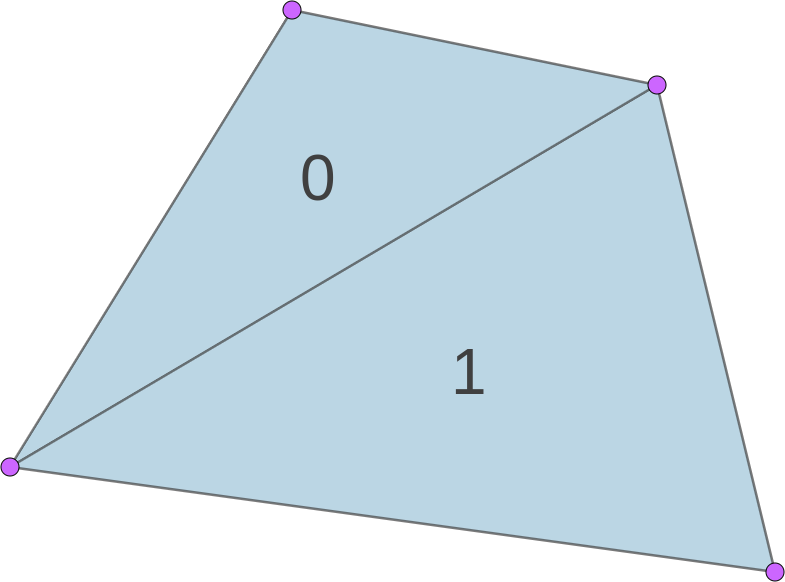
\includegraphics[width = 0.4\linewidth]{Figures/2cell.png}
	\caption{Small two cell example of a mesh.}
	\label{fig:2cell}
\end{figure}
\subsection{Enforcing Boundary Conditions}\label{boundaries}

Boundary conditions have been conveniently ignored up to this point in the report for simplicity's sake when explaining how to assemble the linear system. However, they of course cannot in reality go without being implemented. Thankfully, certain boundary conditions are easier to handle than others. Looking at Equations~\eqref{linsys}, the first term on the right-hand side is a contour integral over the boundary where the Neumann condition applies. Subbing in $g$ into the inner-product here has now in fact dealt with the Neumann condition - this is known as a \textit{natural boundary condition}, where it is handled naturally as part of the integration by parts or Green's lemma.

The Dirichlet conditions on the other hand, are a little more tricky - these must be manually enforced and are thus known as \textit{essential boundary conditions}. Robin conditions contain both essential and natural components so won't be looked at here as these are simply separated into the two components and handled as usual. There are a number of ways of handling the essential boundaries, one would be to restrict your degrees of freedom set $\mathcal{I}_s$, such that it no longer contains any of the nodes which are boundaries and are thus emitted from the stiffness matrix as they are not unknowns, since $A \in \mathbb{R}^{\text{dim} \mathcal{I}_s \times \text{dim}\mathcal{I}_s}$. In this instance, the function being approximated would look like,
\begin{equation}
	u(x) \approx \sum_{j\in\mathcal{I}_b}U_j\varphi_j(x) + \sum_{j\in\mathcal{I}_s}c_j \varphi_{\widetilde j}(x),
\end{equation}
where $\mathcal{I}_b$ is the set of all boundary points, $U_j$ is the boundary value at node $j$ and $\widetilde{j}$ is the updated node index for $\mathcal{I}_s$, less the boundary nodes. This can cause some hassle with bookkeeping as the nodes' indices are being messed around with which can cause headaches when mapping back to the global indices.

Instead of this method, modification of the linear system approach was taken, whereby all nodes remain in the set of unknowns' indices. Since the boundary values are exact solutions at that particular point of the system, the corresponding row and column with that node are set to be all $0$, barring $1$ on the diagonal, and the RHS to be equal to the boundary value. This will force the system to give, $1 \times c_j = U_j \implies u(x_j) = u_j$ for a boundary value at global node number $j$. To achieve this, the element matrices are assembled as normal, and then a four step linear algebra operation is performed,
\begin{enumerate}
	\item $b_i \leftarrow b_i - A_{i,j}U_j\quad\forall i \in \mathcal{I}_s,$
	\item $A_{i,j} = A_{j,i} \leftarrow 0$,
	\item $A_{j,j} \leftarrow 1$,
	\item $b_j \leftarrow U_j$.
\end{enumerate}
Looking at the example in Equation~\ref{elemmat} and Equation~\ref{elemvec}, if supposing an essential boundary condition $U_0$ is enforced at local node $0$, the updated element matrix would be,
\begin{equation}
	\widetilde{A}^{(e)} =
	\left[\begin{matrix} 
		1 & 0 & 0 \\
		0 & \widetilde{A}^{(e)}_{1,1} & \widetilde{A}^{(e)}_{1,2} \\
		0 & \widetilde{A}^{(e)}_{2,1} & \widetilde{A}^{(e)}_{2,2}
	\end{matrix}\right],
\end{equation}
and updated element vector,
\begin{equation}
	\widetilde{b}^{(e)} =
	\left[\begin{matrix}
		U_0 \\
		\widetilde{b}^{(e)}_1 - \widetilde{A}^{(e)}_{0,1} U_0 \\
		\widetilde{b}^{(e)}_2 -\widetilde{A}^{(e)}_{0,2} U_0 \\
	\end{matrix}\right].
\end{equation}
These can now be assembled into the global stiffness matrix and stress vector just as before without any other changes necessary.
\cite{mardal}
\subsection{Physical or Local Coordinates}\label{coords}

The last outstanding piece of mathematics that needs to be touched upon in the FEM is the coordinate mapping of the nodes. In Equation~\ref{linsys}, clearly the integrals or inner-products are all calculated with respect to the physical coordinates of $\mathbf{x}$, across the domain upon which they are defined - compact or whole domain. However, as was mentioned, much of the advantage of the FEM is that you can shape a complex domain into many smaller domains with easier to calculate integrals. In this case, it might be much more within one's interest to locally define the coordinates in each cell and then map back. For example, take a 2D, P1 case again, it might be much more convenient for the node's local coordinates to be (0,0), (0,1) and (1,0) in any cell. For example, to apply this mathematically, denote the local coordinate system by $\mathbf{X}$ and the new, easier local basis functions $\widetilde\varphi_r(\mathbf{X})$, and now consider the integral,
\begin{equation}
	\int_{\Omega^{(e)}} \alpha(\mathbf{x})\nabla \varphi_i(\mathbf{x}) \cdot \nabla \varphi_j(\mathbf{x})~d\mathbf{x}.
\end{equation}
using the transformation,
\begin{equation}
	\nabla_\mathbf{X}\widetilde\varphi_r(\mathbf{X}) = \mathbf{J}\cdot \varphi_i(\mathbf{x}),
\end{equation}
where $\mathbf{J}$ is the Jacobian,
\begin{equation}
	\mathbf{J} =
	\left[\begin{matrix}
		\frac{\partial x_0}{\partial X_0} & \frac{\partial x_1}{\partial X_0}\\
		\frac{\partial x_0}{\partial X_0} & \frac{\partial x_1}{\partial X_1}
	\end{matrix}\right].
\end{equation}
Subbing these in results in the equivalency,
\begin{equation}
	\int_{\Omega^{(e)}} \alpha(x)\nabla \varphi_i(\mathbf{x}) \cdot \nabla \varphi_i(\mathbf{x})~d\mathbf{x} = \int_{\widetilde{\Omega}^{(e)}} \alpha(\mathbf{x}(\mathbf{X}))(\mathbf{J}^{-1}\cdot\nabla_\mathbf{X}~\widetilde\varphi_r(\mathbf{X}) )\cdot(\mathbf{J}^{-1}\cdot\nabla_\mathbf{X}~\widetilde\varphi_s(\mathbf{X}))~\vert\mathbf{J}\vert~d\mathbf{X},
\end{equation}
where ${\widetilde{\Omega}^{(e)}} = [0,1]\times[0,1]$. This mapping can easily be performed on all of the terms in Equation~\eqref{linsys}. The clear advantage here is, previously the basis functions were written as Lagrange polynomials, now since the range of values only spans from 0 to 1,
\begin{align}
	\widetilde\varphi_0(\mathbf{X}) &= 1 - X_0 - X_1,\\
	\widetilde\varphi_1(\mathbf{X}) &= X_0,\\
	\widetilde\varphi_2(\mathbf{X}) &= X_1,
\end{align}
thus leaving far easier integrals to evaluate.~\cite{mardal}

\section{Implemented Example}

\subsection{Problem Statement}\label{problem}
	Given that the intent of this paper is to investigate novel approaches to solving PDEs using the FEM on GPUs, it wouldn't make much sense to code a very complicated PDE for testing purposes. Instead, the 2D Laplace equation was used with a standard rectangular boundary -  mainly as it is non-transient/steady state. It is defined as,
\begin{align}
	\nabla\cdot(\alpha\nabla u(\mathbf{x})) &= 0,\quad \mathbf{x}\in \Omega, \\
	u(\mathbf{x}) &= U_0,\quad \mathbf{x} \in \Gamma_{D0},\\
	u(\mathbf{x}) &= U_1,\quad \mathbf{x} = \Gamma_{D1},\\
	\frac{\partial u}{\partial \mathbf{n}} &= 0,\quad \mathbf{x} \in {\Gamma_N},
\end{align}
where
\begin{align*}
	\Omega &= [a,c]\times[b,d],\\
	\Gamma_{D_0} &= \{\mathbf{x} : x_0 = a\},\\
	\Gamma_{D_1} &= \{\mathbf{x} : x_0 = b\},\\
	\Gamma_N &= \{\mathbf{x} : x_1 = c~||~x_1 = d\}.
\end{align*}
This, when converted into its weak formulation by Green's identity gives,
\begin{align}
	\int_\Omega \nabla\cdot(\alpha\nabla u(\mathbf{x}))~v~d\mathbf{x} &= -\int_\Omega \alpha\nabla u \cdot \nabla v~d\mathbf{x} + \int_{\Gamma_N} \alpha \frac{\partial u}{\partial \mathbf{n}},\\
	&= -\int_\Omega \alpha\nabla u \cdot \nabla v~d\mathbf{x}.
\end{align}
So it can be said that,
\begin{align}
	A_{i,j} &= \left\langle \alpha \nabla \varphi_j, \nabla \varphi_i\right\rangle\label{lhs}\\
	b_i &= 0.
\end{align}
\begin{figure}
	\centering
	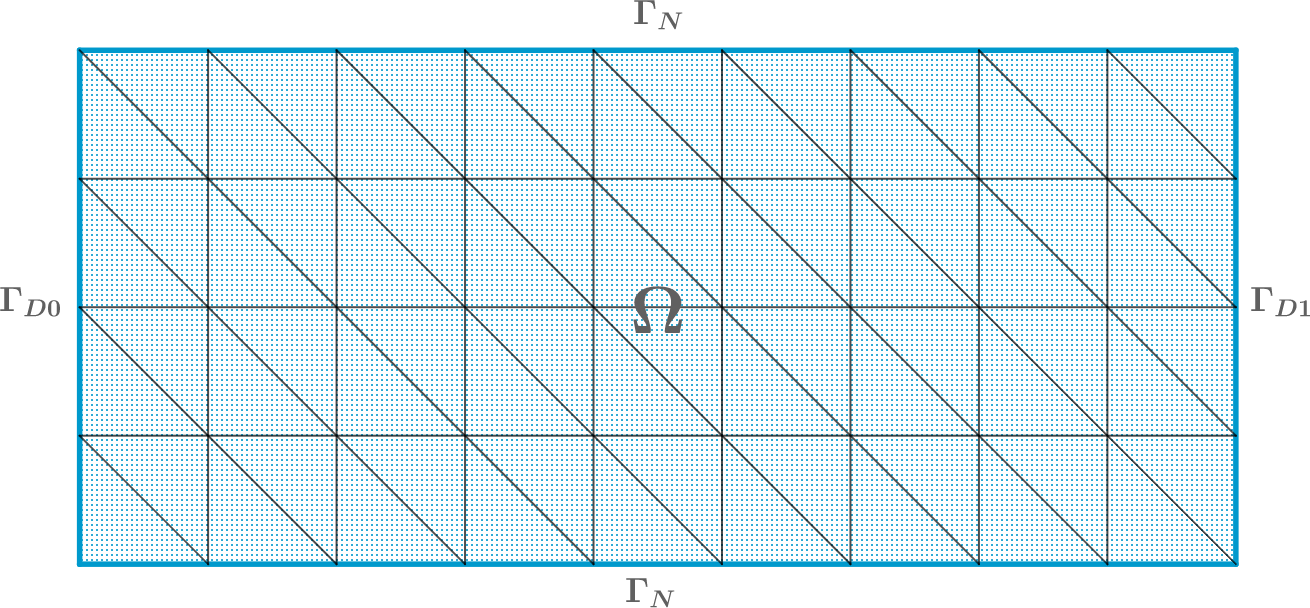
\includegraphics[width = 0.65\linewidth]{Figures/domain}
	\caption{Domain of the Laplace problem to be solved.}
	\label{fig:domain}
\end{figure}
Figure~\ref{fig:domain} demonstrates the mesh being arranged into downward sloping, triangular cells where the node numbering is done in anti-clockwise direction to maintain orientation of the integrals. For more convenience, for the sake of the paper, to avoid manually calculating the Jacobian and performing numerical integration, as seen in Section~\ref{coords}, P1 problems were used and some handy analytical solutions to Equation~\eqref{lhs} exist which only work for 2D, P1, triangular meshes. If the physical, non-local, coordinates of a nodes in a cell are defined by, $x_i, y_i~\forall i \in \mathcal{I}_s$, then define two constants,
\begin{align}
	\beta_i &= y_j - y_k,\\
	\gamma_i &= x_k - x_j,
\end{align} 
and the area of the cell,
\begin{equation}
	\Delta = \frac{1}{2}\left\vert
	\begin{matrix}
		1 & x_i & y_i \\
		1 & x_j & y_j \\
		1 & x_k & y_k
	\end{matrix}\right\vert.
\end{equation}
Without going into large amounts of detail, it can be deduced mathematically that Equation~\eqref{lhs}, on a compact support,
\begin{align}
	\int_{\Omega^{(e)}} \alpha \nabla \varphi_j \cdot \nabla \varphi_i~d\mathbf{x} &= \int_{\Omega^{(e)}}\frac{\Delta^2}{4}(\beta_i\beta_j + \gamma_i\gamma_j)~d\mathbf{x}\\
	&= \frac{\Delta^3}{4}(\beta_i\beta_j + \gamma_i\gamma_j).\label{conv}
\end{align}
\cite{mardal}

\subsubsection{Analytical Solution}

This given problem has the analytical solution,
\begin{equation}
	u(x,y) = U_1 + \left(\frac{U_1 - U_0}{b - a}\right) (x - a).
\end{equation}
Figure~\ref{fig:soln} illustrates this solution plotted in Wolfram Mathematica.
\begin{figure}
	\centering
	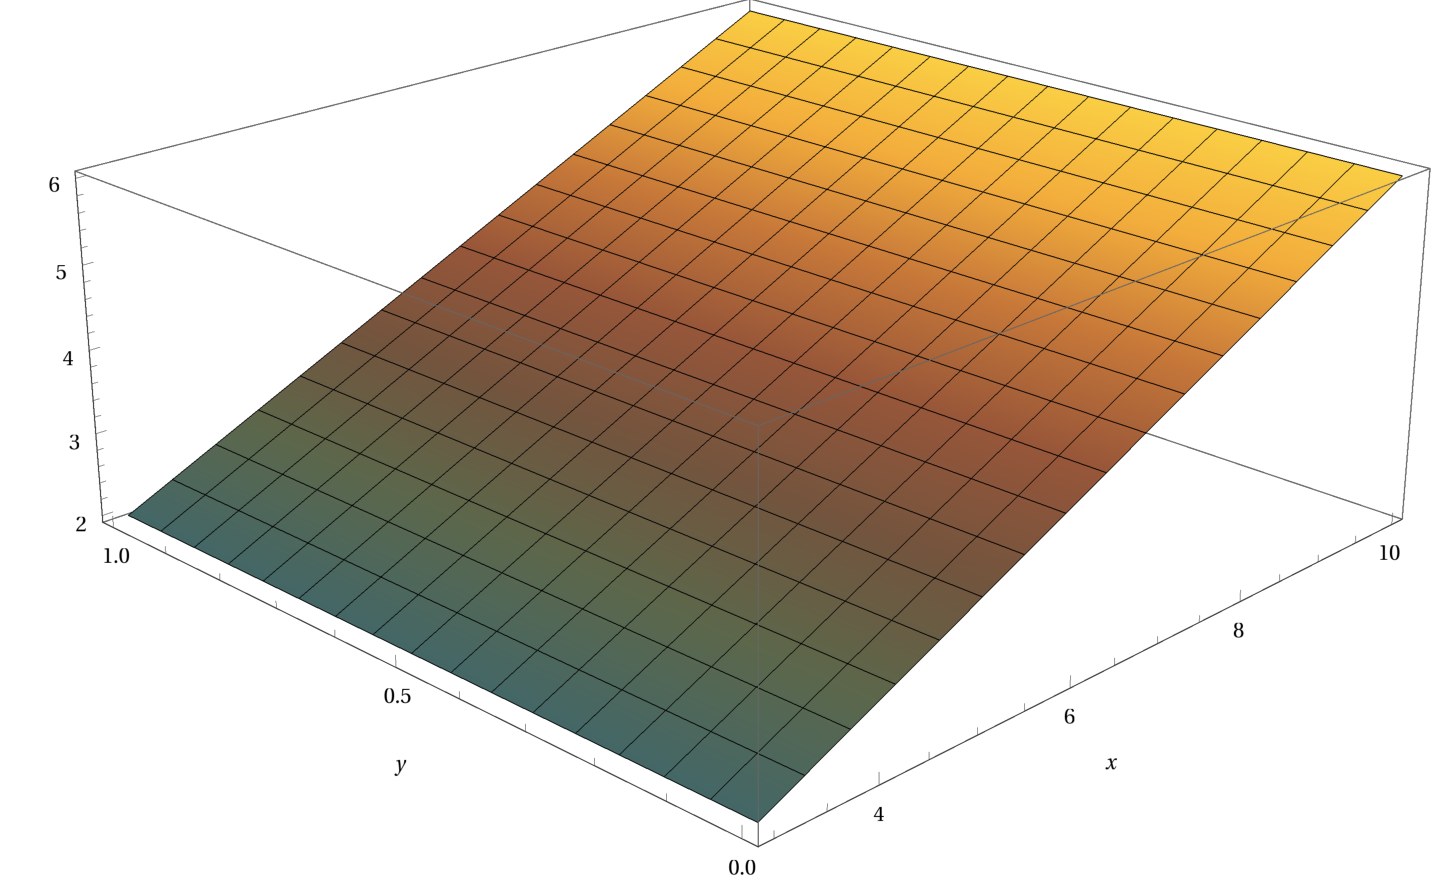
\includegraphics[width=0.6\linewidth]{Figures/soln}
	\caption{Plot of solution to PDE problem posed.}
	\label{fig:soln}
\end{figure}

%See Figure \ref{fig:UoC} for details. Additional information can be
%found in the footnote \footnote{Image taken from \url{https://en.wikipedia.org/wiki/File:Siegel_Uni-Koeln_(Grau).svg}.}.
